\documentclass[11pt, aspectratio=169]{beamer}

\usetheme[progressbar=frametitle, numbering=fraction]{metropolis}
\setbeamercolor{background canvas}{bg=white}

\usepackage{multirow}
\usepackage{graphicx}
\graphicspath{{./figures}}
\usepackage{booktabs}
\usepackage{caption}

\newcommand{\guesser}{\texttt{Guesser}}
\newcommand{\enquirer}{\texttt{Enquirer}}
\newcommand{\rimgscale}{0.7}
\newcommand{\vimgscale}{0.8}

\title{Interactive Speaker Recognition}
\author{Vyacheslav Golovin \texorpdfstring{\newline}{, }
    {\small Aleksandr Samarin (supervisor)}}
\institute[HSE]{Huawei CBG AI and HSE University}
\date{June 22, 2023}


\begin{document}

\maketitle

\begin{frame}{Introduction}
    \textbf{Speaker recognition} (SR) is the task of recognizing a person using
    speech audio. There are 2 types of SR tasks:
    \begin{enumerate}
        \item \textbf{Identification} --- select a speaker from a group.
        \item \textbf{Verification} --- decide whether the selected person
        is the actual speaker.
    \end{enumerate}

    In deep learning setting both these tasks come down to comparing speaker
    and speech vector representations, which we will refer to as
    \alert{speaker} and \alert{word embeddings}.
\end{frame}

\begin{frame}{Motivation}
    \textbf{Application:} Speaker verification system which prompts the speaker
    to say some word or phrase in order to verify their identity.

    \textbf{Requirements:}
    \begin{itemize}
        \item few (short) prompts,
        \item high accuracy,
        \item diverse prompts to avoid spoofing.
    \end{itemize}

    \textbf{Proposal:} select requested words with a neural network trained
    using reinforcement learning.\vspace{1em}

    \begin{quote}
        \normalfont{}
        \emph{A Machine of Few Words --- Interactive
        Speaker Recognition with Reinforcement Learning}, Mathieu Seurin et al.,
        INTERSPEECH 2020, \texttt{arXiv:2008.03127v1}.
    \end{quote}

\end{frame}

\begin{frame}{Interactive Speaker Recognition}
    Input data: TIMIT dataset (630 speakers, 20 shared words).

    Audio is processed with MFCC and x-vector neural network.

    \begin{columns}[c]
        \column{0.6\textwidth}
        \begin{figure}[bht]
            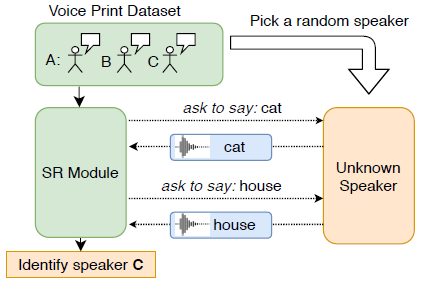
\includegraphics[scale=\rimgscale]{isr_game.png}
        \end{figure}

        \column{0.4\textwidth}
        Important notes:
        \begin{enumerate}
            \item Only identification problem is considered.
            \item The set of words is fixed.
            \item SR Module uses 2 separate neural networks: \enquirer{} and
            \guesser{}.
        \end{enumerate}
        \end{columns}
\end{frame}

\begin{frame}{\guesser{}}
    \begin{figure}[bht]
    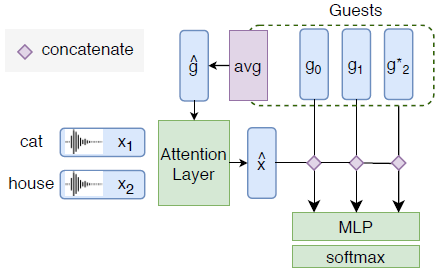
\includegraphics[scale=\rimgscale]{guesser.png}%
    \end{figure}

    \begin{columns}[t]
        \column{.4\textwidth}
        Inputs:
        \begin{itemize}
            \item speaker embeddings $g_k$
            \item word embeddings $x_t$
        \end{itemize}

        \column{.5\textwidth}
        Outputs:
        \begin{itemize}
            \item probability distribution over speakers $P(k = \text{target})$
        \end{itemize}
    \end{columns}
\end{frame}

\begin{frame}{\enquirer{}}
    \begin{figure}[bht]
        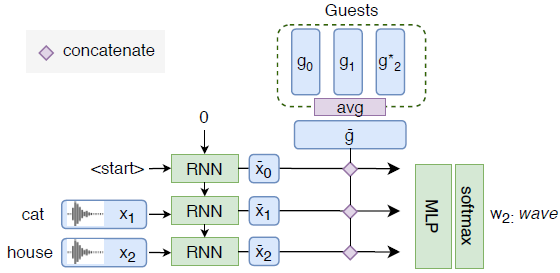
\includegraphics[scale=\rimgscale]{enquirer.png}
    \end{figure}

    \begin{columns}[t]
        \column{.4\textwidth}
        Inputs:
        \begin{itemize}
            \item mean speaker embedding $\hat{g}$
            \item uttered word embeddings $x_t$
        \end{itemize}

        \column{.5\textwidth}
        Outputs:
        \begin{itemize}
            \item probability distribution over vocabulary $P(v =
            \text{requested word})$
        \end{itemize}
    \end{columns}
\end{frame}

\begin{frame}[t]{Training \guesser{}}
    \begin{columns}
        \centering
        \column{.5\textwidth}
        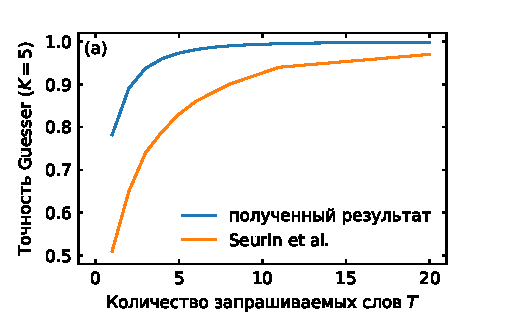
\includegraphics[scale=\vimgscale]{../plots/word_sweep.pdf}
        \column{.5\textwidth}
        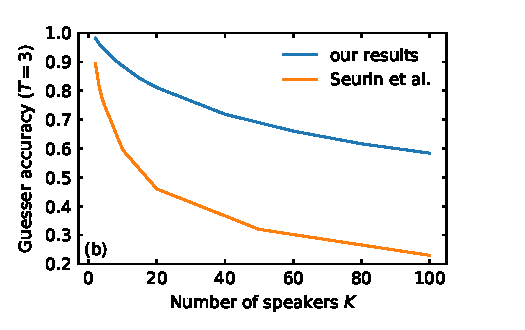
\includegraphics[scale=\vimgscale]{../plots/guest_sweep.pdf}
    \end{columns}

    Here and henceforth the models are trained with $K = 5$ speakers and
    $T = 3$ requested words. \guesser{} is trained with supervised learning ---
    speakers and requested words are randomly sampled.

    The difference is likely due to the increase in embedding size --- 512 vs
    128 in the original paper.
\end{frame}

\begin{frame}[t]{Training \enquirer{}}
    \begin{columns}
        \centering
        \column{.5\textwidth}
        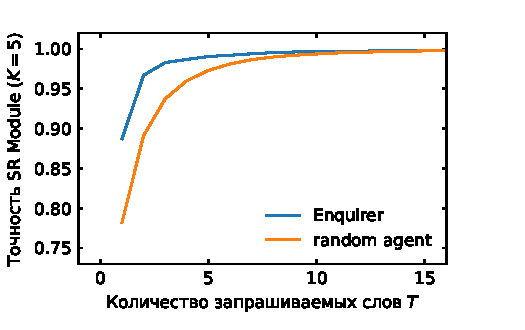
\includegraphics[scale=\vimgscale]{../plots/word_sweep_enq.pdf}
        \column{.5\textwidth}
        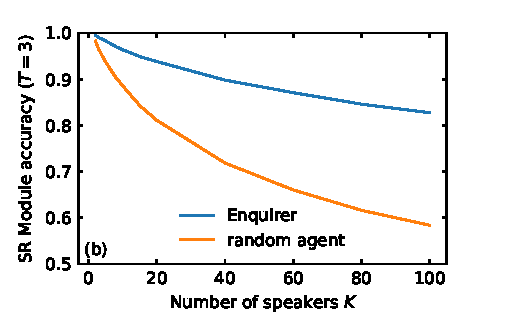
\includegraphics[scale=\vimgscale]{../plots/guest_sweep_enq.pdf}
    \end{columns}

    Trained with reinforcement leaning, namely \textbf{PPO} algorithm.
    \enquirer{} selects words for trained \guesser{}, reward of $1.0$ is received
    if \guesser{} correctly chooses target speaker.
\end{frame}

\begin{frame}{Heuristic agent}
    \begin{columns}[b]
        \column{.3\textwidth}
        \begin{figure}[htb]
            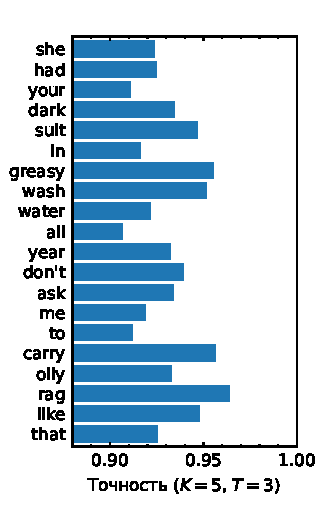
\includegraphics[scale=\vimgscale]{../plots/word_scores.pdf}
        \end{figure}
        \column{.7\textwidth}
        \begin{enumerate}
            \item Compute word accuracies on validation subset.
            \item Sample only from a subset of words with the highest accuracies.
        \end{enumerate}
        \begin{figure}[htb]
            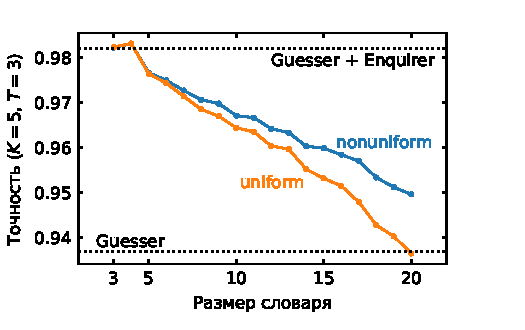
\includegraphics[scale=\vimgscale]{../plots/heuristic.pdf}
        \end{figure}
    \end{columns}
\end{frame}

\begin{frame}[t]{\enquirer{} vs heuristic agent}
    \begin{columns}
        \centering
        \column{.5\textwidth}
        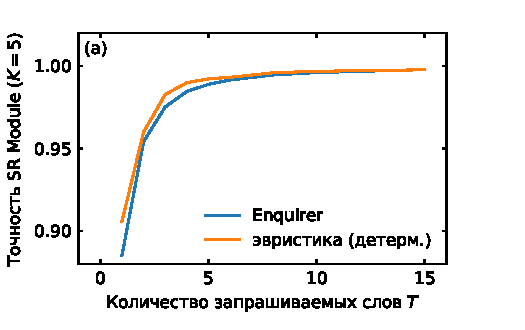
\includegraphics[scale=\vimgscale]{../plots/word_sweep_heuristic.pdf}
        \column{.5\textwidth}
        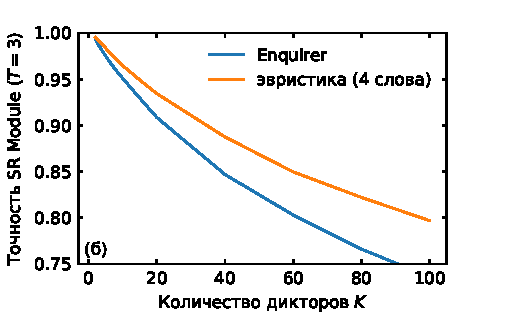
\includegraphics[scale=\vimgscale]{../plots/guest_sweep_heuristic.pdf}
    \end{columns}

    The two agents' policies are very similar, i.e., \enquirer{} mostly selects
    the same words irrespective of guest composition, more diverse policies
    typically perform worse.
\end{frame}

\begin{frame}{From identification to verification}
    \begin{columns}
        \column{.7\textwidth}
        \begin{figure}[bht]
            \only<1>{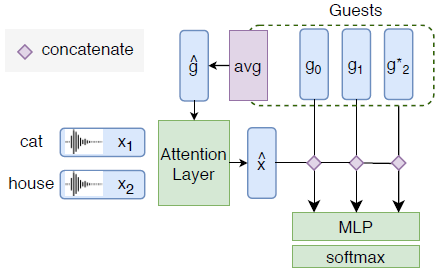
\includegraphics[scale=\rimgscale]{guesser.png}}
            \only<2,3>{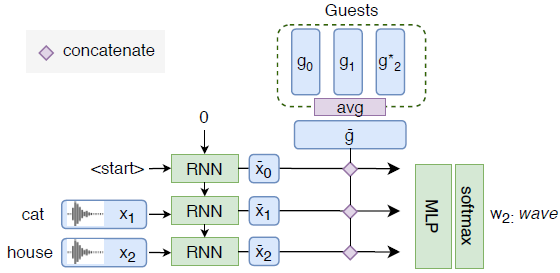
\includegraphics[scale=\rimgscale]{enquirer.png}}
        \end{figure}
        \column{.3\textwidth}
        \begin{itemize}
            \item<1-> \guesser{}: replace softmax with sigmoid
            \item<2-> \enquirer{}: no changes required
        \end{itemize}\vspace{1em}

        \only<3> {
            \begin{tabular}{c c}
                \toprule
                Agent & Accuracy\\
                \midrule
                random & 0.895\\
                Enquirer & 0.933\\
                heuristic & 0.917\\
                \bottomrule
            \end{tabular}
        }
    \end{columns}
\end{frame}

\begin{frame}{Selecting the training mode}
    \only<2>{
        \begin{table}[htb]
            \begin{tabular}{c c c}
                \toprule
                Agent & Training mode & Accuracy\\
                \midrule
                random & \multirow{3}{4em}{$K = 5$\newline$T = 3$} & 0.937 \\
                Enquirer & & 0.982\\
                heuristic & & 0.984\\
                \midrule
                random & \multirow{3}{4em}{$K = 20$\\$T = 2$} & 0.951 \\
                Enquirer & & 0.989\\
                heuristic & & 0.988\\
                \bottomrule
            \end{tabular}
            \caption*{Identification accuracy, $K = 5$ speakers, $T = 3$
                      requested words}
        \end{table}
    }
    \only<1>{
        \begin{table}[htb]
            \begin{tabular}{c c c}
                \toprule
                Agent & Training mode & Accuracy\\
                \midrule
                random & \multirow{3}{4em}{$T = 3$} & 0.895 \\
                Enquirer & & 0.933\\
                heuristic & & 0.917\\
                \midrule
                random & \multirow{3}{4em}{$T = 2$} & 0.913 \\
                Enquirer & & 0.947\\
                heuristic & & 0.945\\
                \bottomrule
            \end{tabular}
            \caption*{Verification accuracy, $T = 3$ requested words}
        \end{table}
    }
\end{frame}

\begin{frame}{\texttt{CodebookEnquirer}}
    \textbf{Problem:} Current \enquirer{} implementation uses a fixed set of
    words. Adding a new one would require retraining or fine-tuning.

    \textbf{Proposed solution:}
    \begin{itemize}
        \item Change last layers of \enquirer{}, so that it returns requested
        word embedding instead of probability distribution.
        \item Construct \texttt{Codebook} --- a tensor of word embeddings
        averaged over training set speakers.
        \item Select next requested word based on distances between output
        and codebook vectors.
    \end{itemize}

    \textbf{Result:} Little to none accuracy penalty, even if different sets of
    words are used during training and testing.
\end{frame}

\begin{frame}{Other experiments}
    \begin{enumerate}
        \item Background noise

        \begin{itemize}
            \item 6 noise samples from MUSAN (rain, car, crowd, typing, hum,
            white) added to word audio with 3~dB SNR\@. Noise type is
            consistent throughout the ISR game episode.
            \item No significant change in results, only a small drop in
            accuracy for every word selection algorithm. Notably, no noise
            adaptation of \enquirer{}.
        \end{itemize}

        \item Different embeddings\vspace{.5em}

        \begin{table}[bht]
            \begin{tabular}{c c c c c}
                \toprule
                \multirow{2}{5em}{Embeddings}
                    & \multicolumn{2}{c}{Identification}
                    & \multicolumn{2}{c}{Verification}\\
                & random & Enquirer & random & Enquirer\\
                \midrule
                x-vector & 0.75 & 0.91 & 0.89 & 0.94\\
                CPC & 0.95 & 0.99 & 0.95 & 0.97\\
                \bottomrule
            \end{tabular}
            \caption*{Speaker recognition accuracy, $K$ = 20 speakers,
                      $T$ = 2 requested words}
        \end{table}

    \end{enumerate}
\end{frame}

\begin{frame}{Conclusions}
    \begin{itemize}
        \item The interactive speaker recognition method works --- selecting
        requested words with a neural agent allows for a significant increase
        in speaker recognition accuracy.
        \item The approach is rather flexible --- we were able to easily
        transition from identification to verification and perform other
        modifications that improve model usability and performance.
        \item Performance is very similar to a simple baseline --- not clear if
        the use of complicated reinforcement learning algorithms is actually
        justified.
    \end{itemize}
\end{frame}

\end{document}
